\documentclass[tikz,border=4pt]{standalone}
\usepackage{lmodern}
\usepackage[T1]{fontenc}
\usepackage{amssymb}
\usetikzlibrary{positioning,fit,arrows.meta,calc,matrix}
\begin{document}
\begin{tikzpicture}[
  font=\footnotesize,
  tok/.style={draw, rounded corners=1pt, minimum height=5.2mm, minimum width=6.6mm, inner sep=1pt, font=\footnotesize\ttfamily},
  multi/.style={tok, fill=orange!25},
  idx/.style={draw, minimum height=5.2mm, minimum width=6.6mm, inner sep=1pt, fill=gray!10},
  lab/.style={font=\footnotesize\bfseries, anchor=west},
  note/.style={font=\scriptsize, text=black!65, align=left, anchor=west},
  arr/.style={-{Latex[length=2mm]}, thick, black!60},
  cell/.style={draw, minimum size=2.6mm, inner sep=0pt, line width=0.2pt, draw=black!40},
  one/.style={cell, fill=black!75},
  emb/.style={cell, fill=blue!20},
]
% ---------------------------------------------------------------- (a) molecule + SMILES
\node[anchor=north west] (mol) at (0,0) {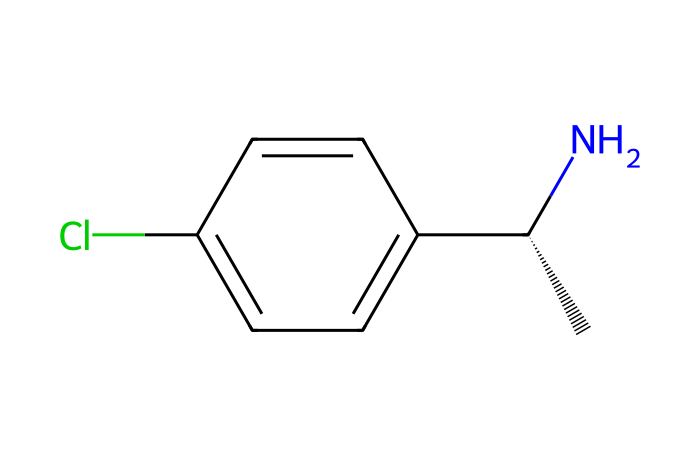
\includegraphics[width=3.1cm]{mol_example.png}};
\node[lab] at ($(mol.north west)+(0,0.35)$) {(a) Molecule and canonical SMILES};
\node[anchor=west, font=\footnotesize\ttfamily] (smi) at ($(mol.east)+(0.3,0.4)$) {C[C@@H](N)c1ccc(Cl)cc1};
\node[note] at ($(smi.west)+(0,-0.5)$) {RDKit canonical form after salt stripping\\and charge neutralisation (22 characters)};
% ---------------------------------------------------------------- (b) tokens
\coordinate (rowb) at (0,-3.3);
\node[lab] at ($(rowb)+(0,0.55)$) {(b) Atom-level tokenisation (16 tokens)};
\foreach \i/\t/\v/\sv in {0/{C}/7/0.09, 1/{[C@@H]}/18/0.23, 2/{(}/5/0.06, 3/{N}/6/0.08, 4/{)}/10/0.13, 5/{c}/3/0.04, 6/{1}/4/0.05, 7/{c}/3/0.04, 8/{c}/3/0.04, 9/{c}/3/0.04, 10/{(}/5/0.06, 11/{Cl}/25/0.32, 12/{)}/10/0.13, 13/{c}/3/0.04, 14/{c}/3/0.04, 15/{1}/4/0.05} {
  \pgfmathsetmacro{\x}{\i*0.78}
  \ifnum\i=1 \node[multi] (t\i) at ($(rowb)+(\x,0)$) {\t};
  \else\ifnum\i=11 \node[multi] (t\i) at ($(rowb)+(\x,0)$) {\t};
  \else \node[tok] (t\i) at ($(rowb)+(\x,0)$) {\t}; \fi\fi
}
\node[note] at ($(t15.east)+(0.25,0.15)$) {regular expression of Schwaller et al.;\\shaded tokens span several characters};
% ---------------------------------------------------------------- (c) vocabulary indices
\coordinate (rowc) at (0,-4.7);
\node[lab] at ($(rowc)+(0,-0.55)$) {(c) Vocabulary lookup ($V=75$ tokens for SIDER; PAD $=0$); arrows map each token to its index};
\foreach \i/\t/\v/\sv in {0/{C}/7/0.09, 1/{[C@@H]}/18/0.23, 2/{(}/5/0.06, 3/{N}/6/0.08, 4/{)}/10/0.13, 5/{c}/3/0.04, 6/{1}/4/0.05, 7/{c}/3/0.04, 8/{c}/3/0.04, 9/{c}/3/0.04, 10/{(}/5/0.06, 11/{Cl}/25/0.32, 12/{)}/10/0.13, 13/{c}/3/0.04, 14/{c}/3/0.04, 15/{1}/4/0.05} {
  \pgfmathsetmacro{\x}{\i*0.78}
  \node[idx] (v\i) at ($(rowc)+(\x,0)$) {\v};
  \draw[arr, thin] (t\i.south) -- (v\i.north);
}
\node[idx, fill=white, densely dashed] (vpad) at ($(rowc)+(16*0.78+0.3,0)$) {0};
\node[note] at ($(vpad.east)+(0.15,0)$) {$\cdots$ padded to $T=198$};
% ---------------------------------------------------------------- (d) three encodings
\coordinate (rowd) at (0,-6.6);
\node[lab] at ($(rowd)+(0,0.5)$) {(d) Three input encodings of the same sequence (first eight positions shown)};
% d1 integer index
\node[note, anchor=north west, text=black] (d1) at ($(rowd)+(0,0.05)$) {\textbf{integer index}\\one scalar $i_t / V$ per position};
\foreach \i/\t/\v/\sv in {0/{C}/7/0.09, 1/{[C@@H]}/18/0.23, 2/{(}/5/0.06, 3/{N}/6/0.08, 4/{)}/10/0.13, 5/{c}/3/0.04, 6/{1}/4/0.05, 7/{c}/3/0.04, 8/{c}/3/0.04, 9/{c}/3/0.04, 10/{(}/5/0.06, 11/{Cl}/25/0.32, 12/{)}/10/0.13, 13/{c}/3/0.04, 14/{c}/3/0.04, 15/{1}/4/0.05} {
  \ifnum\i<8
  \pgfmathsetmacro{\x}{\i*0.62}
  \node[idx, minimum width=5.8mm, font=\tiny] (s\i) at ($(rowd)+(\x+0.3,-1.15)$) {\sv};
  \fi
}
\node[note] at ($(s0.west)+(0,-0.55)$) {shape $T\times 1$; imposes an ordinal\\relation between unrelated tokens};
% d2 one-hot
\coordinate (d2o) at ($(rowd)+(6.3,0)$);
\node[note, anchor=north west, text=black] at ($(d2o)+(0,0.05)$) {\textbf{one-hot}\\binary vector of length $V$\\per position};
\foreach \r in {0,...,9} { \foreach \c in {0,...,7} {
  \node[cell] at ($(d2o)+(0.15+\c*0.27,-1.05-\r*0.27)$) {};
}}
% rows (0..9) stand for vocabulary indices 3,4,5,6,7,10,18,25,...; ones at the index of each token
\foreach \c/\r in {0/4,1/6,2/2,3/3,4/5,5/0,6/1,7/0} { \node[one] at ($(d2o)+(0.15+\c*0.27,-1.05-\r*0.27)$) {}; }
\node[note] at ($(d2o)+(0,-4.05)$) {shape $T\times V$; sparse, fixed width};
% d3 embedding
\coordinate (d3o) at ($(rowd)+(10.3,0)$);
\node[note, anchor=north west, text=black] at ($(d3o)+(0,0.05)$) {\textbf{learned embedding}\\trainable table $E\in\mathbb{R}^{V\times d}$,\\row $E[i_t]$ per position};
\foreach \r in {0,...,4} { \foreach \c in {0,...,7} {
  \pgfmathsetmacro{\sh}{15+mod(\r*37+\c*53+\r*\c*11,55)}
  \node[cell, fill=blue!\sh] at ($(d3o)+(0.15+\c*0.27,-1.05-\r*0.27)$) {};
}}
\node[note] at ($(d3o)+(0,-2.9)$) {shape $T\times d$ ($d=64$ default, 16--128 searched);\\dense, learned jointly with the network};
% arrows to network
\node[draw, rounded corners=2pt, fill=gray!8, minimum height=6mm, align=center] (net) at ($(rowd)+(7.3,-4.9)$) {convolution / recurrent layers $\rightarrow$ classifier};
\draw[arr] ($(s3.south)+(0,-0.85)$) -- (net.north west);
\draw[arr] ($(d2o)+(1.2,-4.3)$) -- (net.north);
\draw[arr] ($(d3o)+(1.2,-3.45)$) -- (net.north east);
\end{tikzpicture}
\end{document}
